\documentclass[10pt]{exam}
\usepackage[hon]{template-for-exam}
\usepackage{tikz,graphicx}

\title{YAPP [Yet Another Practice Problem]}
\author{Rohrbach}
\date{\today}

\begin{document}
\maketitle

\vspace{1em}

\begin{center}
  \begin{tikzpicture}
    \node at (-.8,0) 
      {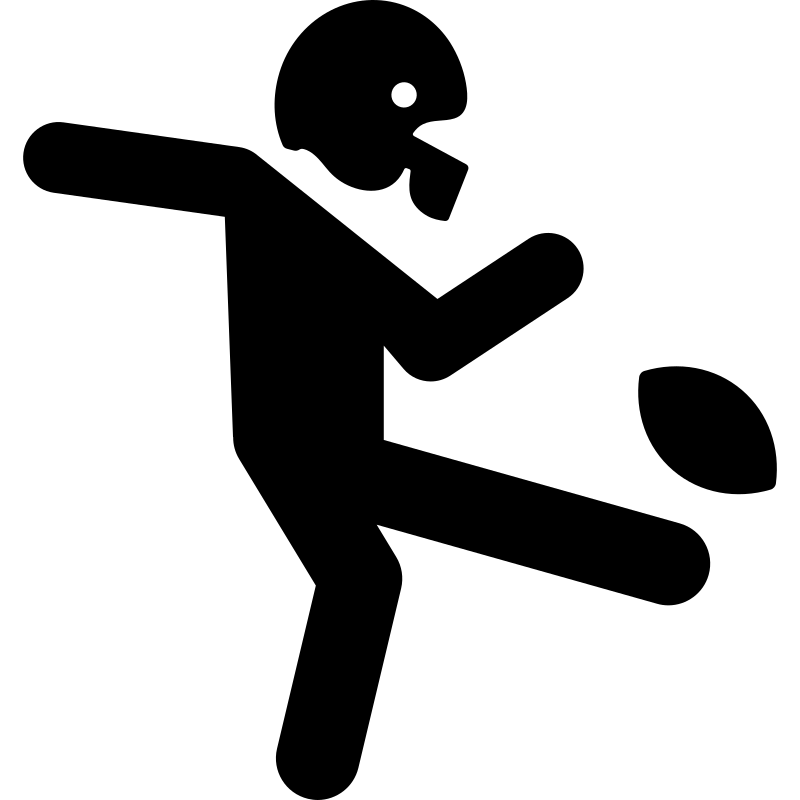
\includegraphics[width=1.5cm]{punter}};
    \draw[dashed,brown] (5,3) parabola (0,0);
    \draw[dashed,brown] (5,3) parabola (10,0);
    \draw[->,thick,red] (-0.1,0) -- ++(50:1.5);
  \end{tikzpicture}
\end{center}


\noindent
A football is kicked at an angle off the ground (as shown in the picture above). The football is in the air for 1.2 seconds and travels forward 53 meters.

\vspace{1em}

\begin{parts}
  \part
    Calculate the $x$- and $y$- components of the football's initial velocity.
  \part
    Use these $x$- and $y$- components to calculate the direction (angle) and magnitude of the football's initial resultant velocity vector.
\end{parts}

\end{document}